\documentclass[10pt]{beamer}

\usetheme[progressbar=foot]{metropolis}
\usepackage{appendixnumberbeamer}

\usepackage{booktabs}
\usepackage[scale=2]{ccicons}

\usepackage{pgfplots}
\usepgfplotslibrary{dateplot}

\usepackage{xspace}
\newcommand{\themename}{\textbf{\textsc{metropolis}}\xspace}

\usepackage{tikz}

\usepackage{wrapfig}

\usepackage{appendixnumberbeamer}

\usepackage{selinput}
\usepackage{ulem}

\usepackage{tabularx}
\usepackage{subcaption}



\title{Variational Autoencoders}
\subtitle{Learning generative models with latent representations}
\date{April 30, 2019}
\author{Claas Völcker}
\institute{Deep Generative Models - SoSe 2019}
% \titlegraphic{\hfill\includegraphics[height=1.5cm]{logo.pdf}}

\begin{document}
%\setlength{\metropolis@progressinheadfoot@linewidth}{100pt}

\maketitle


\begin{frame}{Table of contents}
\setbeamertemplate{section in toc}[sections numbered]
\tableofcontents[hideallsubsections]
\end{frame}


\section{Inference through optimization}

\begin{frame}{What if we replaced an inference question with optimization?}
    \begin{itemize}[<+->]
        \item The target: $$P(X)$$
        \item The hope: there is a nice $$z,~\text{so that}~P(X) = \int P(z)P(X|z)dz$$ which governs X (latent variable)
        \item i.e. all dogs look similar, if I know something is a dog, certain attributes (tails, legs, snout) are likely
        \item idea: rephrase inference as optimization
    \end{itemize}
\end{frame}

%\begin{frame}{But we know nothing about it!}
%    \begin{itemize}
%        \item How does knowing about z help us?
%    \end{itemize}
%    \begin{gather}
%        \max_\phi \sum_x p(\phi, x)\\
%        = \max_\phi \sum_x \log p(\phi, x)\\
%        = \max_\phi \sum_x \log \int p(z) p_\phi(x | z) dz
%    \end{gather}
%    \begin{gather}
%        \sum_x \int \log \frac{p_\phi(z | x) \cdot p_\phi(x)}{p_\phi(z)}
%    \end{gather}
%\end{frame}

\begin{frame}{Working through the math - 1}

    \begin{gather}
        \text{Maximize: }P(X) \sim \int p_\phi(X|z)p_\phi(z)dz
    \end{gather}
    \begin{itemize}[<+(1)->]
        \item a latent variable model
        \item Assumption: there is some (hopefully small) z which governs data
        \item define $P(z)$, $P(X|z)$ and $\int$?
        \item first intuition: choose ``easy'' $P(z)$ (like Gaussian), learn $P(X|z)$ from the data
    \end{itemize}
    \pause
    \begin{gather}
        P(X|z) = \mathcal{N}(X|f(z;\phi),\sigma^2 \cdot I)
    \end{gather}

    \begin{itemize}[<+->]
        \item $f$ is deterministic, $\mathcal{N}$ enables optimization
    \end{itemize}
\end{frame}

\begin{frame}{Working through the math - 2}
    \begin{itemize}[<+->]
        \item We could maximize by sampling?
        \item No, too many samples would be needed
        \item A given $z$ is never guaranteed to produce a likely $X$
        \item We are sampling far from the useful mainfold
        \item $P(Z|X)$ is intractable, it is the reverse of what we are looking for
        \item We need to learn a surrogate probability density $Q(Z)$
        \item $Q(Z)$ should be close to $P(Z|X)$
    \end{itemize}
    \end{frame}

    \begin{frame}{Working through the math - 3}
    \begin{gather}
        \mathcal{KL}[Q(Z)||P(Z|X)] = \mathbb{E}_{z\sim Q}[\log Q(Z) - \log P(Z|X)]
    \end{gather}
    \pause
    \begin{itemize}
        \item Using Bayes rule:
    \end{itemize}
        \pause
    \begin{gather}
        \mathcal{KL}[Q(Z)||P(Z|X)] = \mathbb{E}_{Z\sim Q}[\log Q(Z) - \log \frac{P(X|Z) P(Z)}{P(X)}]\\
        = \mathbb{E}_{Z\sim Q}[\log Q(Z) - (\log P(X|Z) + \log P(Z) - \log P(X))]\\
        = \mathbb{E}_{Z\sim Q}[\log Q(Z) - \log P(X|Z) - \log P(Z)] + \log P(X)
    \end{gather}

\end{frame}

\begin{frame}{Working through the math - 4}
    \begin{gather}
        \mathcal{KL}[Q(Z)||P(Z|X)] = \mathbb{E}_{Z\sim Q}[\log Q(Z) - \log P(X|Z) - \log P(Z)] + \log P(X)\\
        \log P(X) - \mathcal{KL}[Q(Z)||P(Z|X)] = \mathbb{E}_{Z\sim Q}[\log P(X|Z)] - \mathcal{KL}[Q(Z)||P(Z)]
    \end{gather}
    \pause

    What we have now:
    \begin{itemize}[<+->]
        \item $\log P(X)$: maximization goal
        \item $\mathcal{KL}[Q(Z)||P(Z|X)$: ``closeness'' of Q to P
        \item $\mathbb{E}_{Z \sim Q}[\log P(X|Z)]$: maximization of $P(X|Z)$ with regards to Q
        \item $\mathcal{KL}[Q(Z)||P(Z)]$: regularization of Q on prior $P(z)$
    \end{itemize}

    \begin{itemize}[<+->]
        \item We can choose Q arbitrarily...
        \item ... so we can choose an entry which depends on x
    \end{itemize}

\end{frame}

\begin{frame}{Working through the math - 5}
    \begin{gather}
        \log P(X) - D[Q(Z|X)||P(Z|X)] = \mathbb{E}_{Z\sim Q}[\log P(X|z)] - D[Q(z|X)||P(z)]
    \end{gather}
    
    \begin{itemize}[<+->]
        \item right hand side: ELBO (Evidence Lower BOund): maximization target
        \item $P(X|z)$ and $Q(z|X)$: decoder and encoder learned from the data
        \item $P(z)$: prior on latent variables
        \item $P(z|X)$ will hopefully be approximated well by $Q(z|X)$. (discussion later)
    \end{itemize}
\end{frame}
\begin{frame}{Working through the math - 6}
    \begin{itemize}[<+->]
        \item Can we optimize now?
        \item No, not yet: we still need to choose $Q(Z|X)$ and work out some math
    \end{itemize}
    \pause
    \begin{gather}
        Q(z|X) = \mathcal{N}(z|\mu(X;\theta),\Sigma(x;\theta))
    \end{gather}

    \begin{itemize}[<+->]
        \item $Q(Z|X)$ can now approximate arbitrary PDF via $\mu$
        \item $\Sigma$ represents noise
    \end{itemize}
\end{frame}

\begin{frame}{Final math slide!}
    \begin{itemize}[<+->]
        \item with choices, ($P(X|Z)\sim\mathcal{N}$ and $Q(Z|X)\sim\mathcal{N}$), KL has closed form solution
            \begin{itemize}
                \item possible for other PDFs too
            \end{itemize}
        \item KL depends on learnable functions $f$ and $\mu$
        \item We can use neural networks to approximate those!
        \item Are we finished now?
    \end{itemize}
\end{frame}

\section{Variational Autoencoders}

\begin{frame}{What is an autoencoder?}
	\begin{center}
            \begin{figure}
                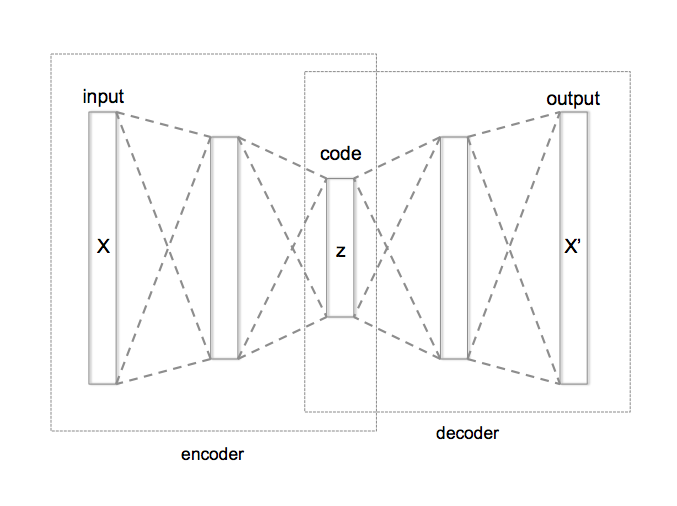
\includegraphics[height=.7\textheight]{figs/Autoencoder_structure.png}
                \caption{Taken from \url{https://commons.wikimedia.org/wiki/File:Autoencoder_structure.png}, (CC BY-SA 4.0)}
            \end{figure}
	\end{center}
\end{frame}

\begin{frame}{What is a variational autoencoder?}
	\begin{center}
            \begin{figure}
                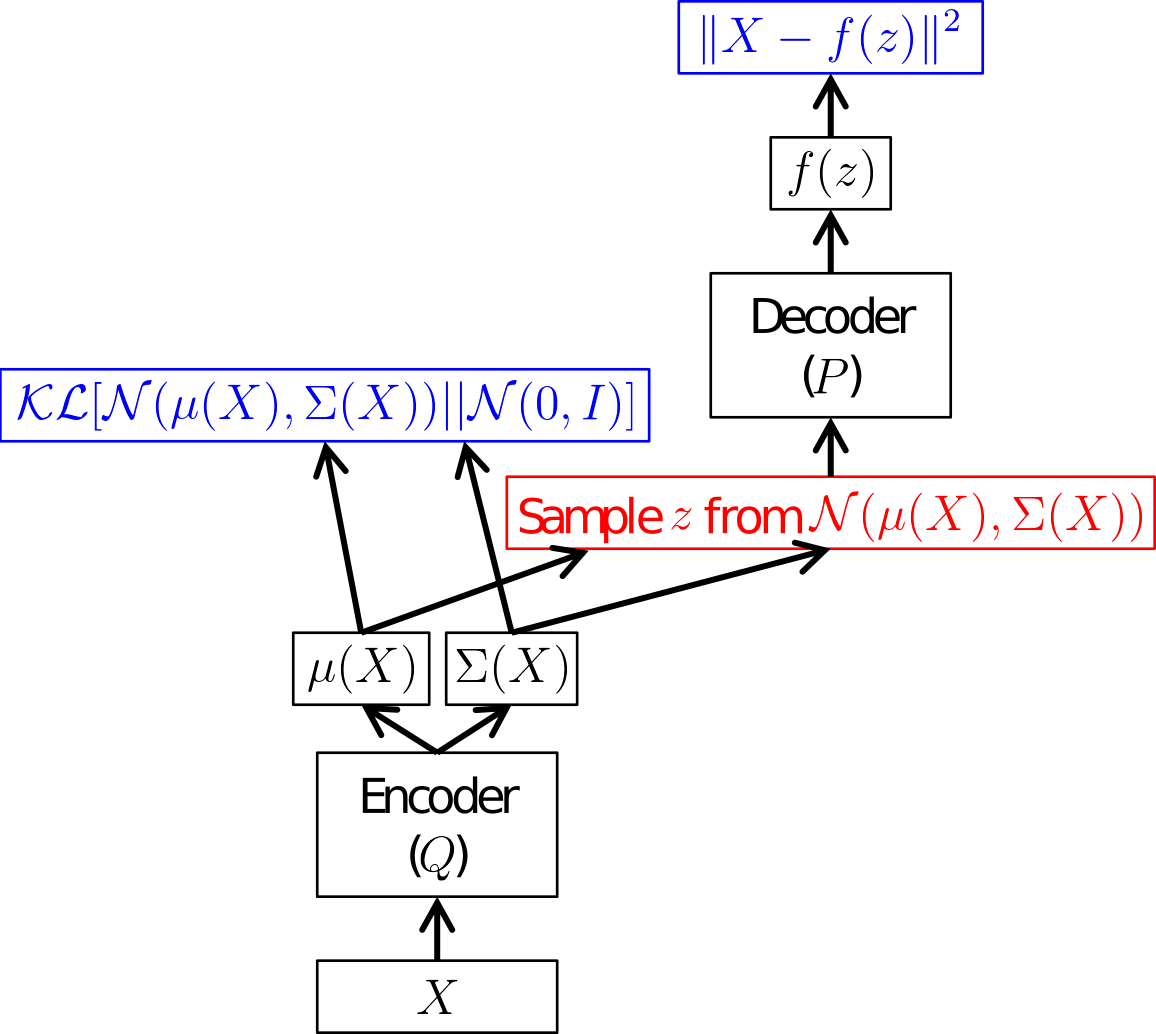
\includegraphics[height=.8\textheight]{figs/net.png}
                \caption{Taken from "Auto-Encoding Variational Bayes", Kingma \& Welling, 2014}
            \end{figure}
	\end{center}
\end{frame}

\begin{frame}{Where is the trick?}
    \begin{minipage}[c]{0.3\textwidth}
            \begin{figure}
                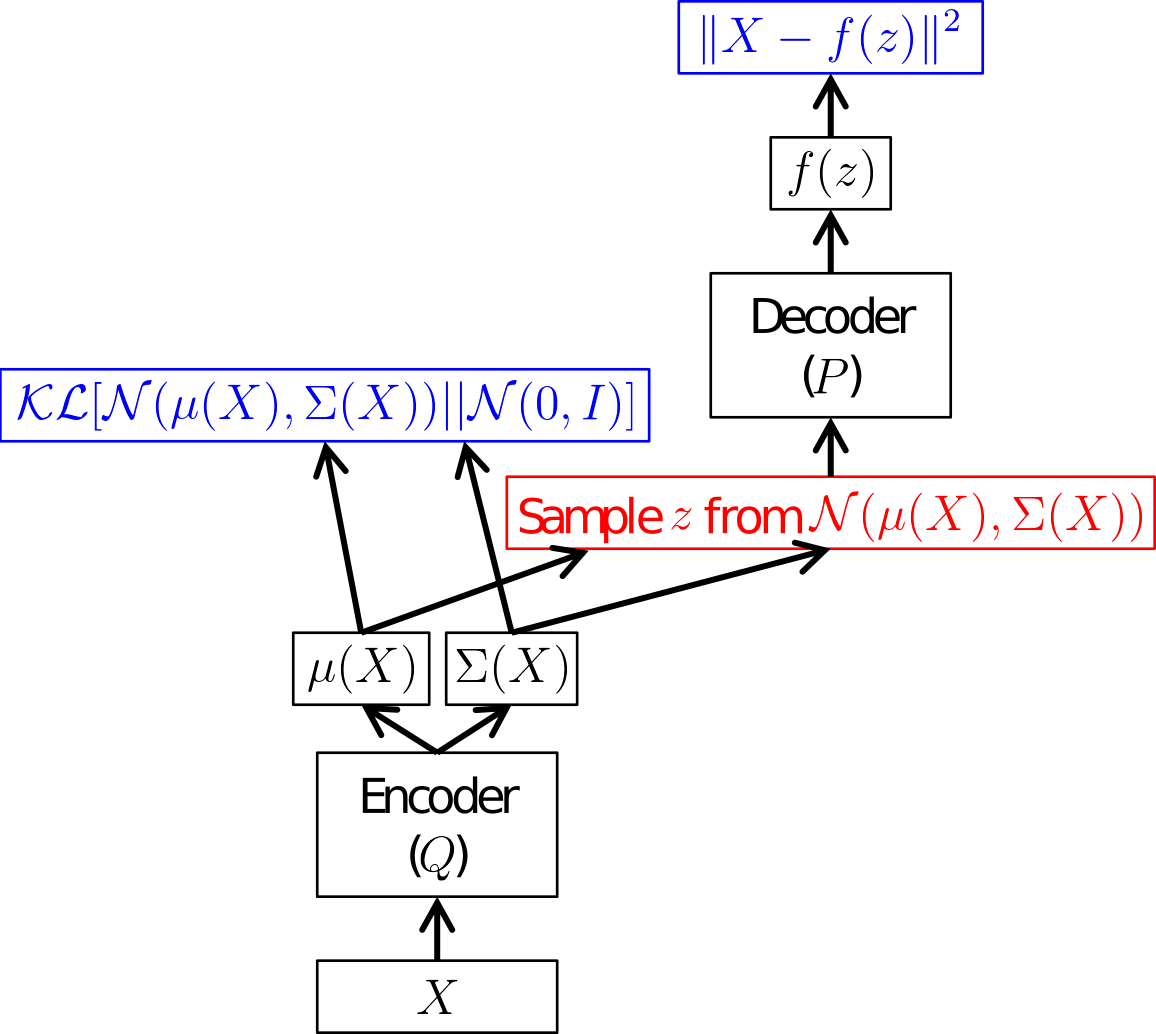
\includegraphics[width=\textwidth]{figs/net.png}
                %\caption{Taken from "Auto-Encoding Variational Bayes", Kingma \& Welling, 2014}
            \end{figure}
    \end{minipage}
    ~
    \begin{minipage}[c]{0.6\textwidth}
        \begin{itemize}[<+(1)->]
            \item ELBO is captured in the optimization by loss
            \item the problem is in backpropagation
            \item you can't propagate through a sampling layer
        \end{itemize}
    \end{minipage}
    
\end{frame}

\begin{frame}{All the parts in detail}
	\begin{center}
            \begin{figure}
                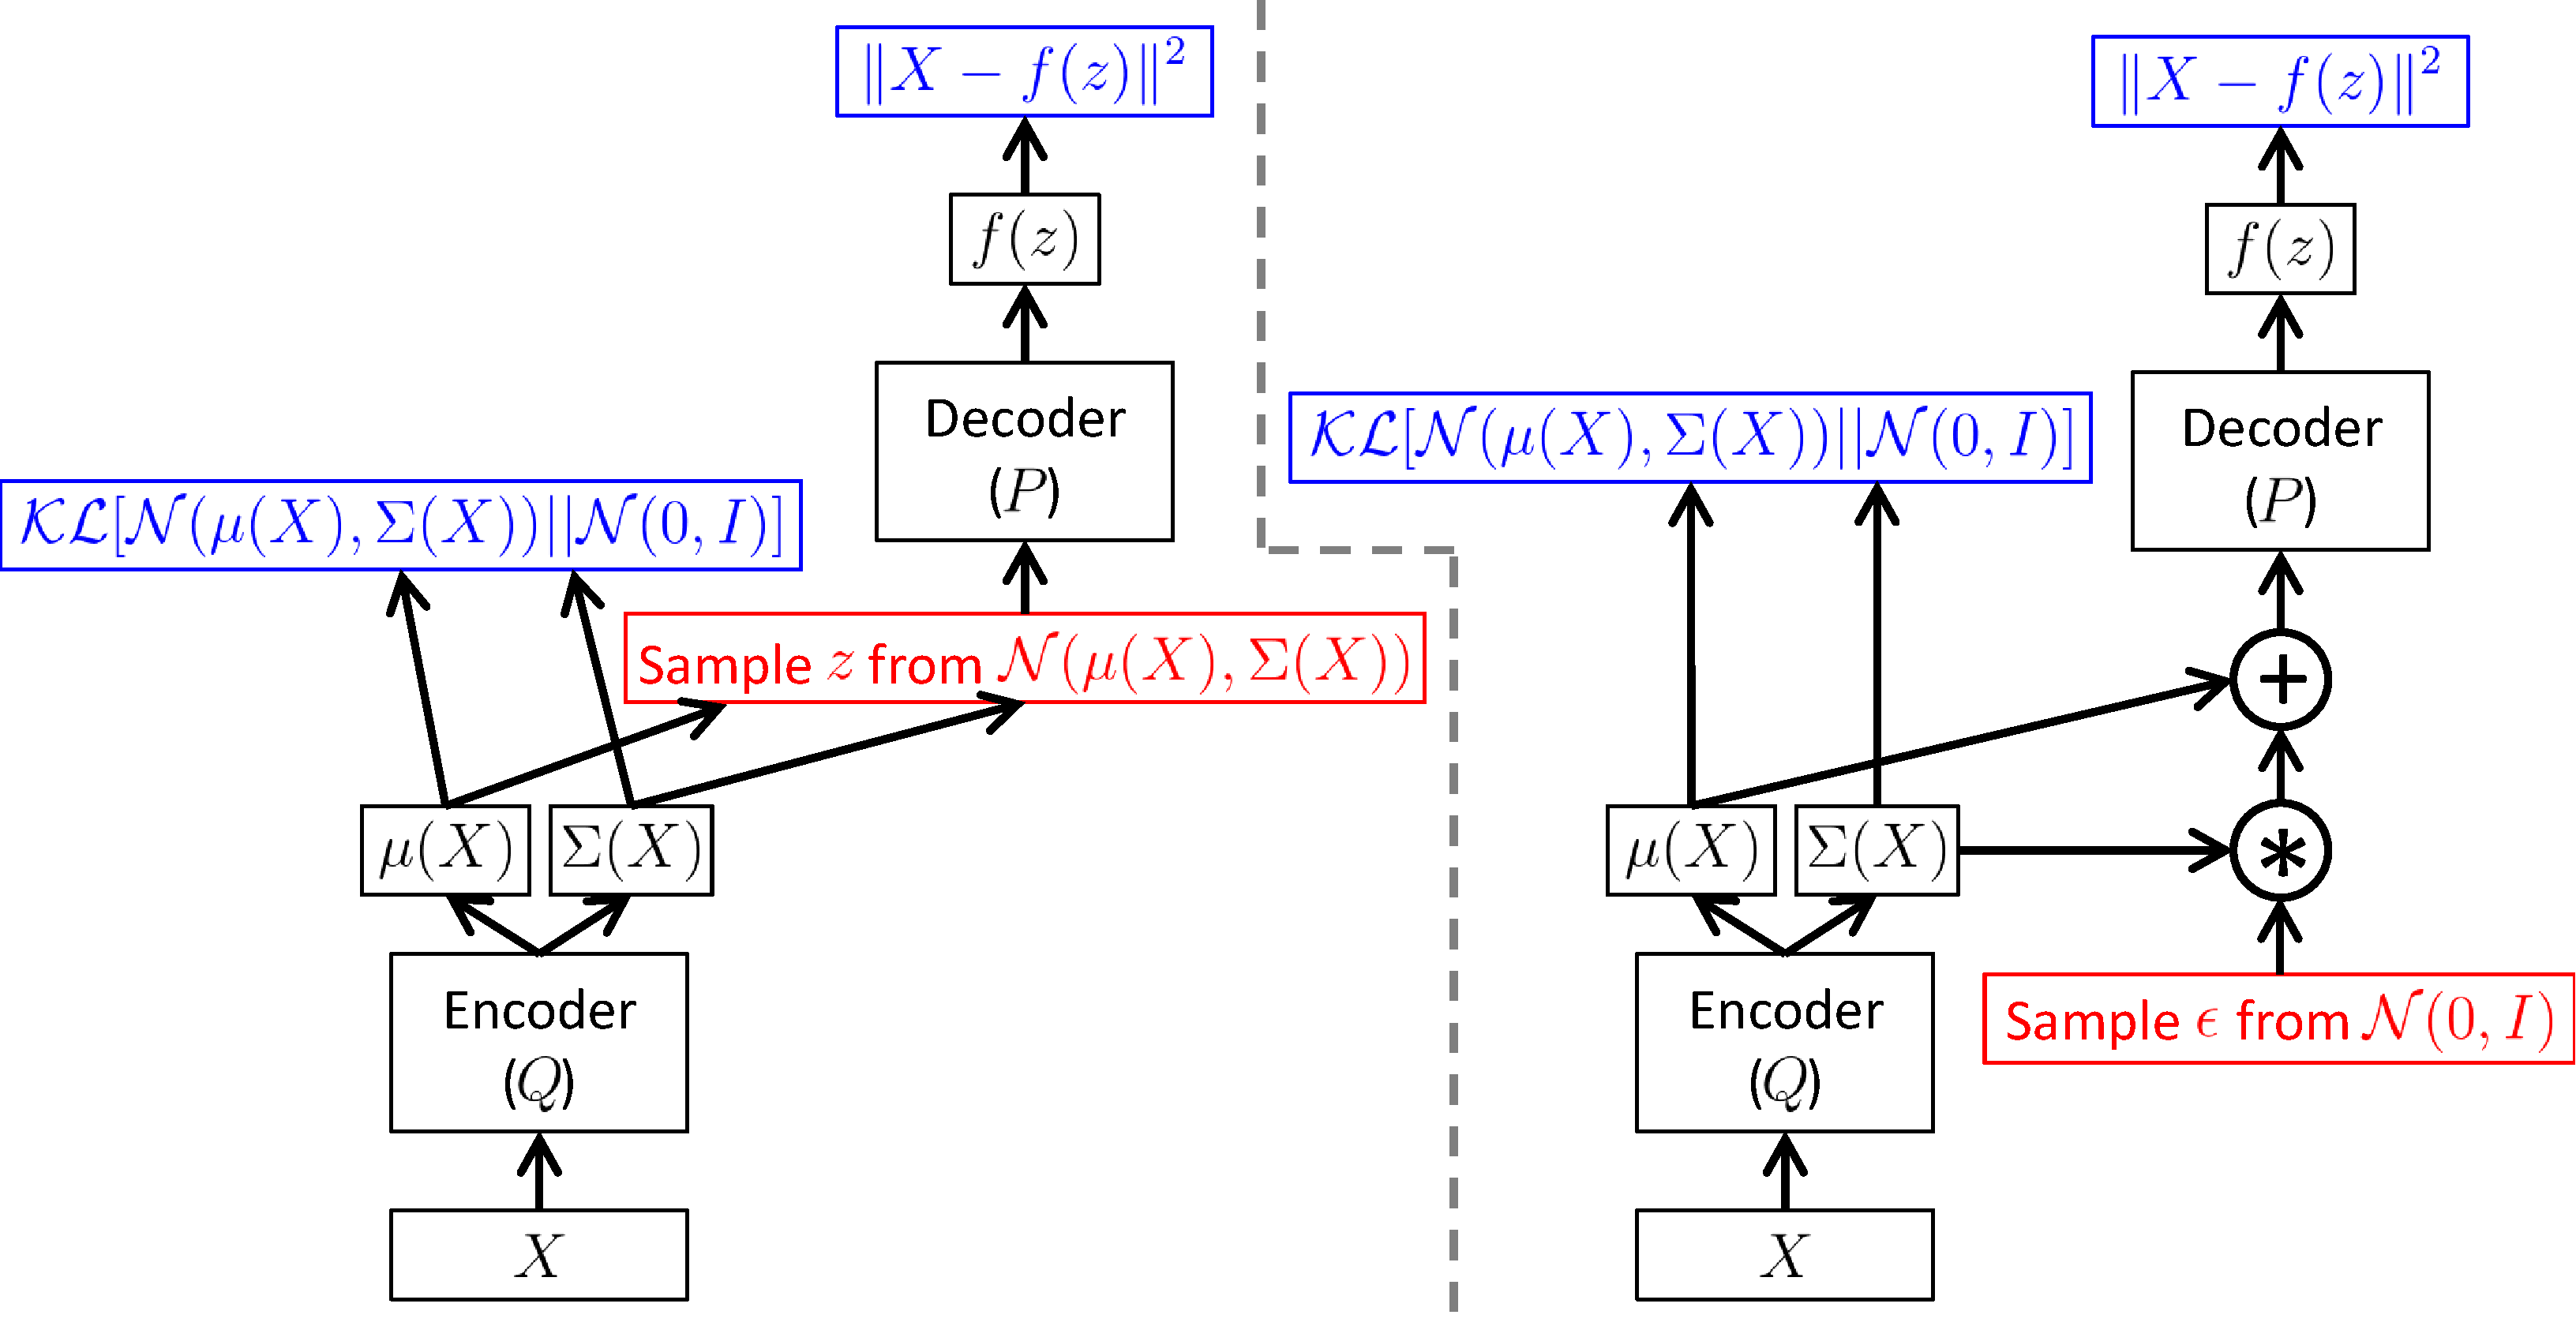
\includegraphics[width=\textwidth]{figs/net.pdf}
                \caption{Taken from "Tutorial on Variational Autoencoders", Doersch, 2016}
            \end{figure}
	\end{center}
\end{frame}

\begin{frame}{Why the sampling at all?}
    \begin{itemize}[<+->]
        \item we are trying to learn a distribution, not an encoder (per se)
        \item encoder - decoder relations are deterministic
        \item how would we sample at inference time?
    \end{itemize}
    \pause
    \begin{center}
        \begin{figure}
            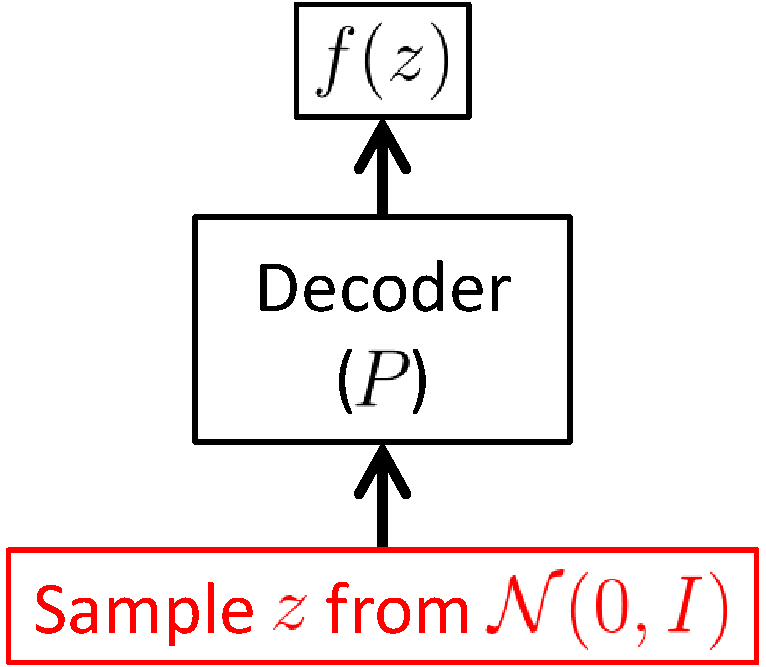
\includegraphics[height=0.4\textheight]{figs/test_time.pdf}
                \caption{Taken from "Tutorial on Variational Autoencoders", Doersch, 2016}
        \end{figure}
    \end{center}
\end{frame}

\begin{frame}[standout]{Code!}
    Code presentation
\end{frame}

\begin{frame}{Why use a variational autoencoder?}
    \begin{itemize}[<+->]
        \item image generation is often done via GAN
        \item is VAE obsolete?
    \end{itemize}
    \pause
    \begin{table}
        \begin{tabularx}{\linewidth}{ l | X X }
            %\hline
            & VAE & GAN \\\hline\hline
            \onslide<+->{Loss & L2 loss & adversarial loss}\\
            \onslide<+->{Latent & structured & unstructured}\\
            \onslide<+->{Results & blurry & sharp}\\
            \onslide<+->{Goal & generate good latent & generate good pictures}
            %\hline
        \end{tabularx}
    \end{table}
    \begin{itemize}[<+->]
        \item VAEs are density models, GAN not so much
        \item but the density is still intractable
        \item there is no mathematical guarantee for choosing a "good" latent
    \end{itemize}
\end{frame}


\section{Applications of VAE}

\begin{frame}{VAE for generating images}
    \begin{figure}
        \begin{subfigure}[c]{0.4\textwidth}
            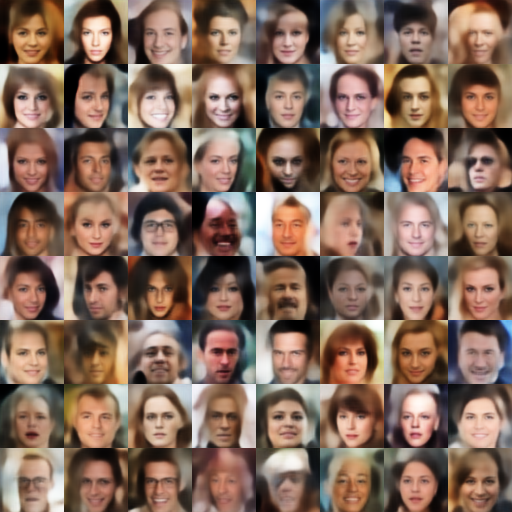
\includegraphics[width=\textwidth]{figs/vae_random.png}
                \caption{Taken from "Tutorial on Variational Autoencoders", Doersch, 2016}
        \end{subfigure}
        ~
        \begin{subfigure}[c]{0.4\textwidth}
            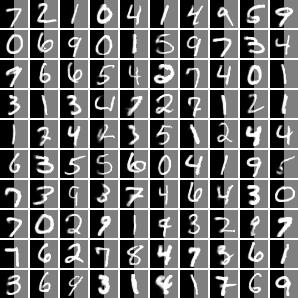
\includegraphics[width=\textwidth]{figs/cvae_out.png}
            \caption{Taken from GitHub \url{https://github.com/yzwxx/vae-celebA}}
        \end{subfigure}
    \end{figure}
\end{frame}

\begin{frame}{VAE for translations}
    \begin{figure}
        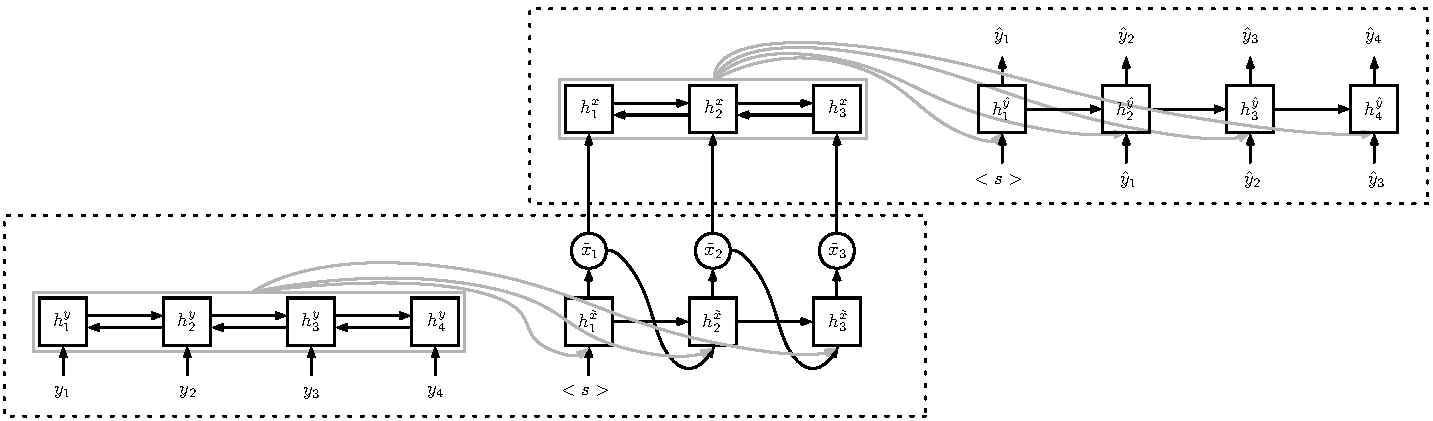
\includegraphics[width=\textwidth]{figs/Seq4model_overview.pdf}
        \caption{Taken from "Semantic Parsing with Semi-Supervised Sequential Autoencoders", Kocisky et al, 2016}
    \end{figure}
\end{frame}

\begin{frame}{More complex VAE usage}
    \begin{figure}
        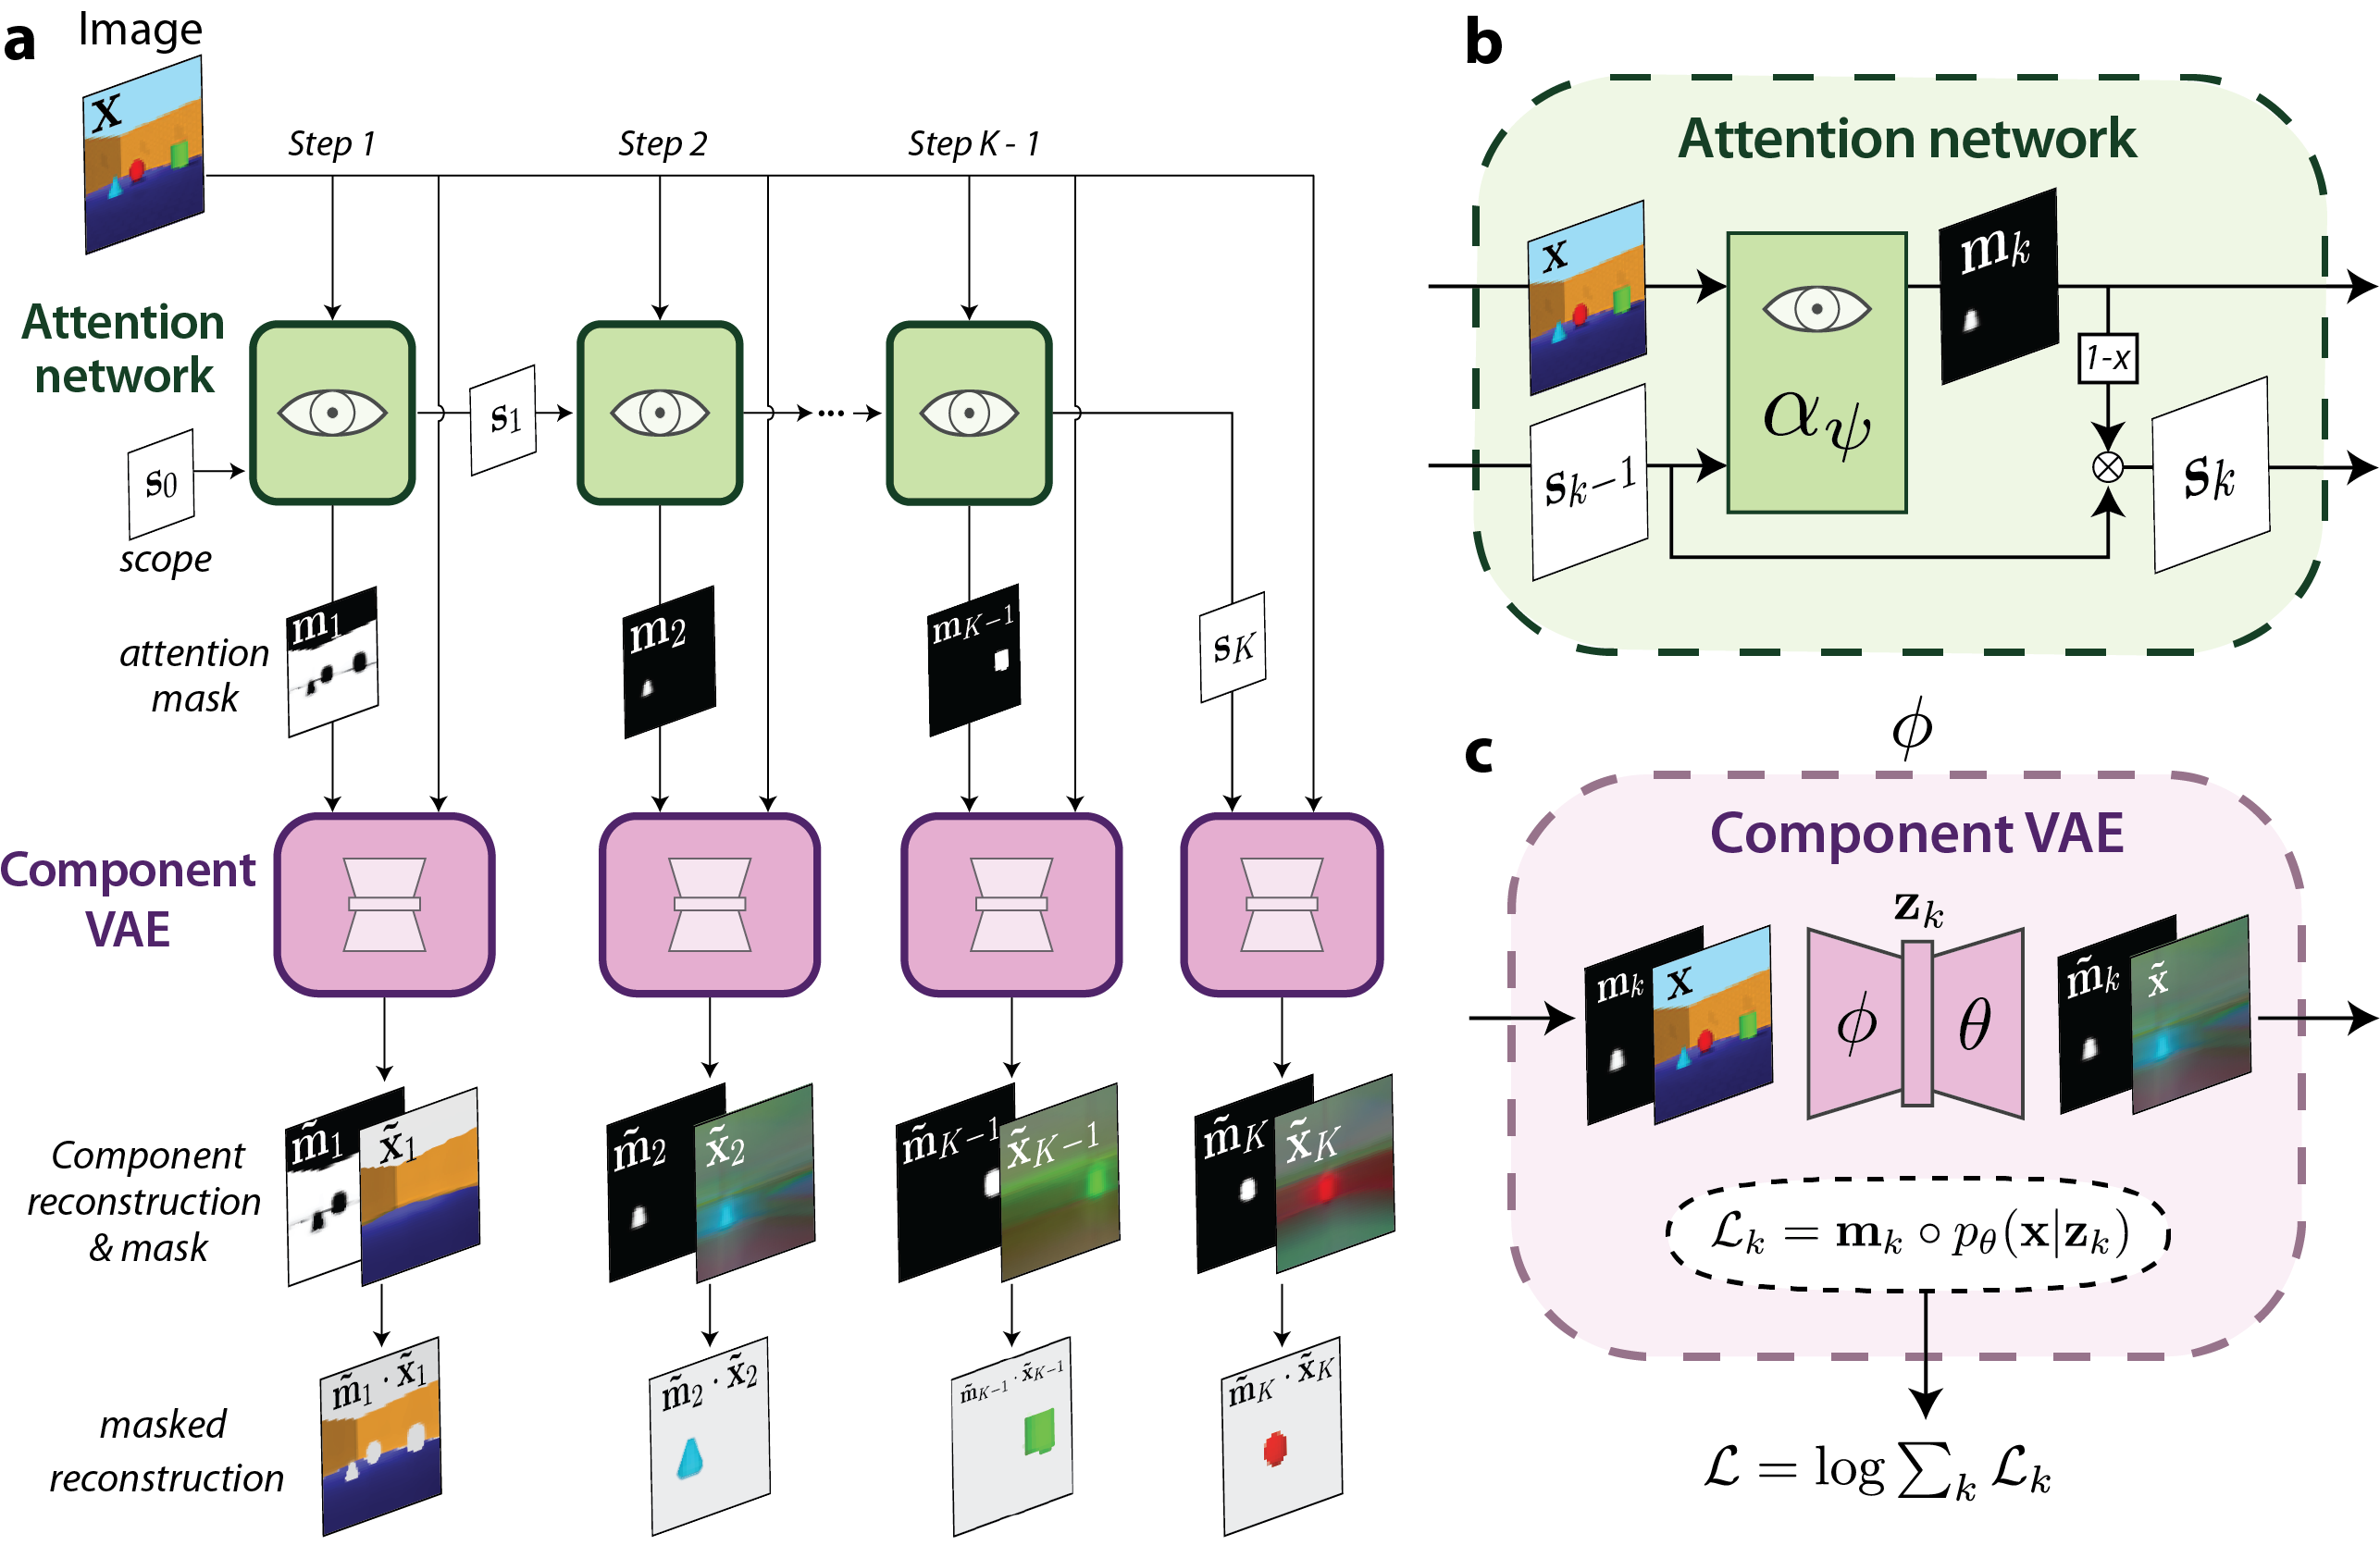
\includegraphics[height=0.7\textheight]{figs/monet_diagram_v2.png}
        \caption{Taken from "MONet: Unsupervised Scene Decomposition and Representation", Burgess et al., 2019}
    \end{figure}
\end{frame}

\begin{frame}{More complex VAE usage}
    \begin{figure}
        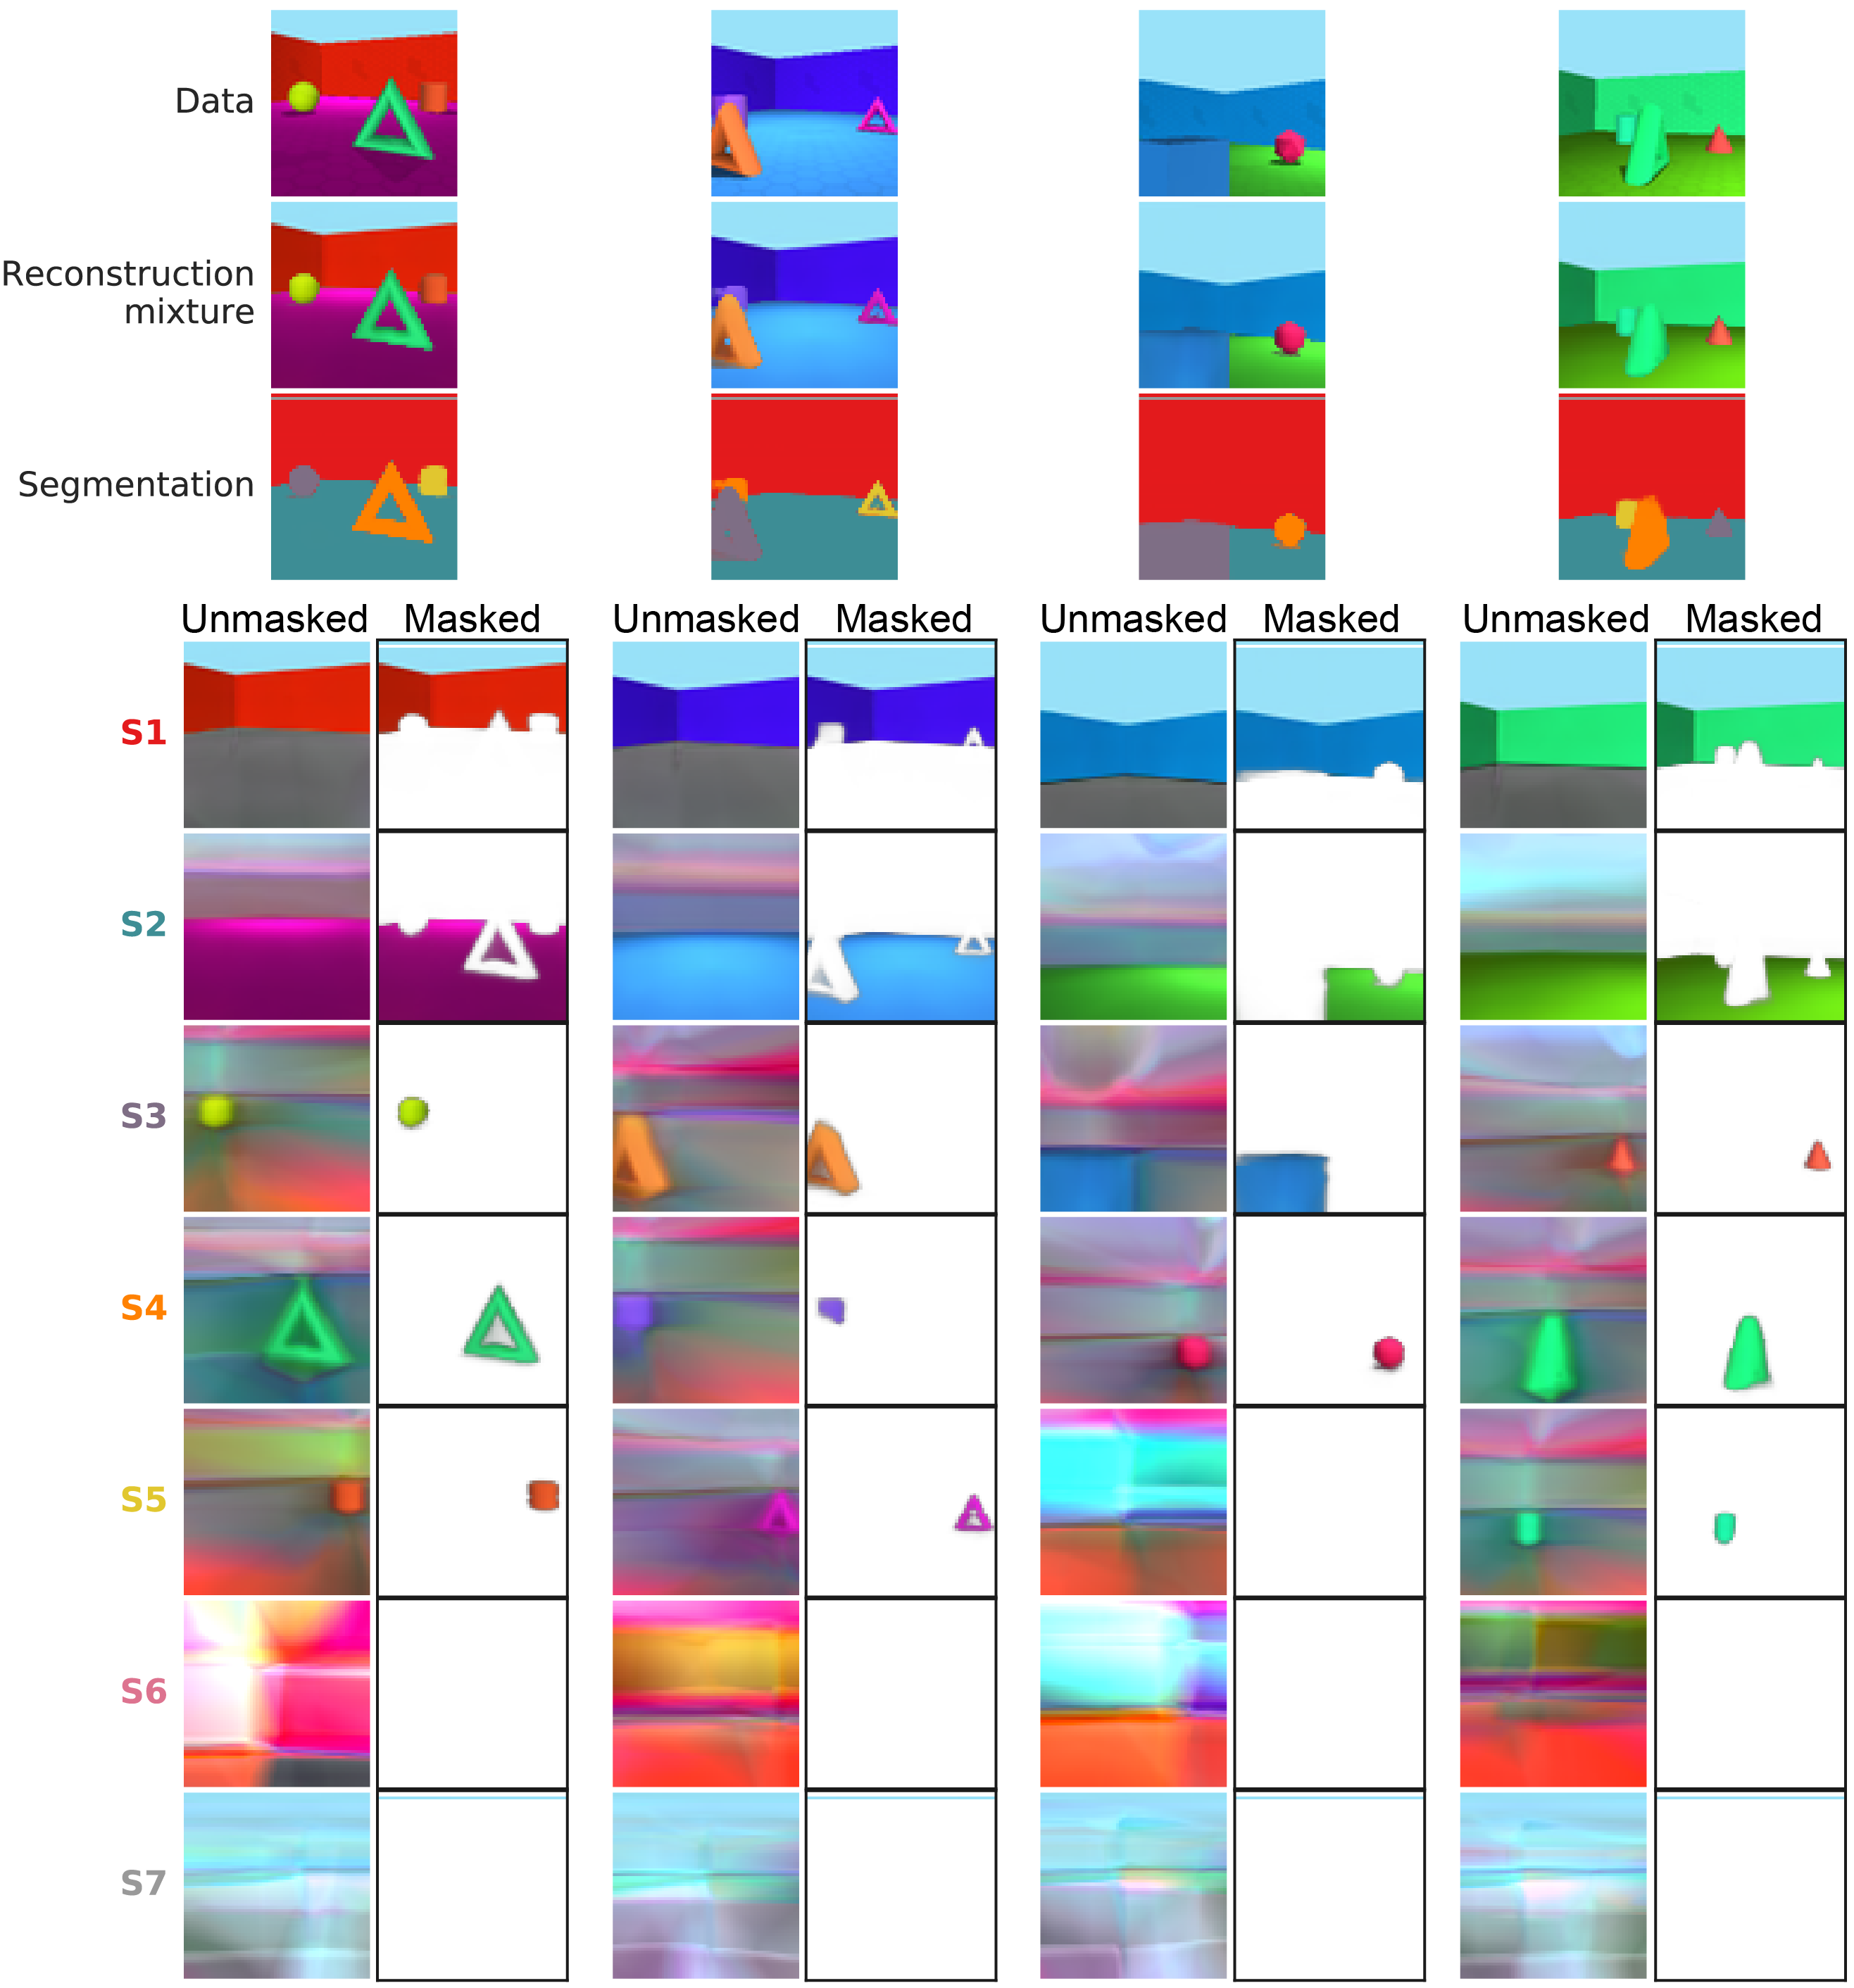
\includegraphics[height=0.7\textheight]{figs/monet_oir_decomposition_masked.png}
        \caption{Taken from "MONet: Unsupervised Scene Decomposition and Representation", Burgess et al., 2019}
    \end{figure}
\end{frame}

\begin{frame}{Further reading}
    \begin{itemize}
        \item "Stochastic Backpropagation and Approximate Inferencein Deep Generative Models" by Danilo Rezende et al., 2014
        \item "Auto-Encoding Variational Bayes" by Durk Kingma and Max Welling, 2014
        \item "Tutorial on Variational Autoencoders" by Carl Doersch, 2016
        \item "Variational Inference: A Review for Statisticians" by David Blei et al., 2018
        \item "Improving Variational Inference with Inverse Autoregressive Flow" by Durk Kingma, 2016
        \item "Attend, Infer, Repeat: Fast Scene Understanding with Generative Models" by Ali Eslami et al., 2016
        \item "The Dreaming Variational Autoencoder for Reinforcement Learning Environments" by Per-Arne Andersen, 2018
    \end{itemize}
\end{frame}

\begin{frame}[standout]{Questions?}
    Any remaining questions?
\end{frame}

\appendix

\begin{frame}{Kullback Leibler Divergence}
    \begin{itemize}
        \item characterizes the "distance" between distributions
        \item positive, 0 only if two distributions are equal (almost everywhere)\footnote{In a mathematical, strict sense, for practical purposes $$KL(P||Q)  = 0~\text{, iff}~ P = Q$$}
        \item not a metric, since it is asymetric, but still useful
    \end{itemize}
    \begin{gather}
        KL(P||Q) = \int p(x) \log\frac{p(x)}{q(x)}dx\\
        = \mathbb{E}_{x\sim p}[\log\frac{p(x)}{q(x)}] = \mathbb{E}_{x\sim p}[\log(p(x)) - \log(q(x))]
    \end{gather}
\end{frame}

\begin{frame}{Kullback Leibler Divergence}
    \begin{center}
        \begin{figure}
            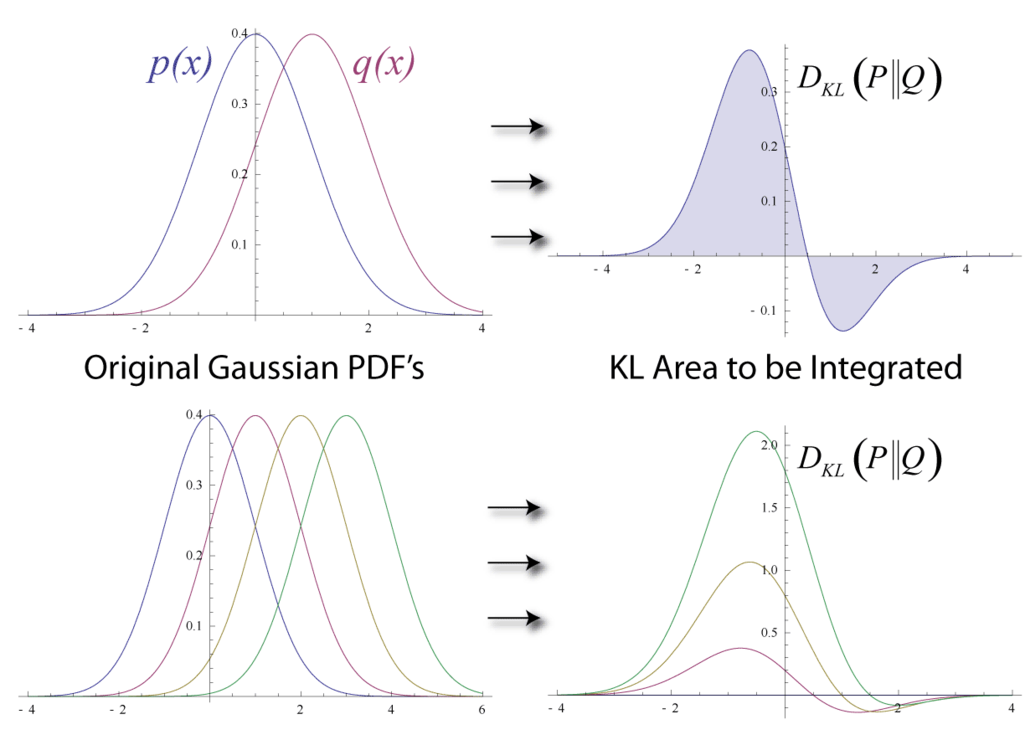
\includegraphics[height=0.8\textheight]{figs/kl.png}
            \caption{Taken from "Kullback–Leibler divergence", Wikipedia, CC BY-SA 3.0}
        \end{figure}
    \end{center}
\end{frame}

\end{document}
